\chapter{Bevezetés}
\usetikzlibrary{shapes,arrows}

\thispagestyle{fancy}
\pagestyle{fancy}
\section{Projekt célja}
A jelenlegi kor társadalmi és technológiai kihívásai közepette egyre fontosabbá válik az emberiség számára az olyan innovatív megoldások keresése, amelyek segíthetnek fejleszteni és támogatni az emberek mindennapi életét. Az Artificial Intelligence (AI), vagyis a Mesterséges Intelligencia, ebben az összefüggésben különösen figyelemre méltó tényezővé vált. Bár sokan aggódnak amiatt, hogy az AI alkalmazása az emberi társadalom hanyatlásához vezethet, én úgy vélem, hogy a megfelelő módon felhasználva az AI lehetőségei elősegíthetik a társadalmi fejlődést és előnyöket hozhatnak az emberi élet számos területén.

Szakdolgozatom központi célja az, hogy az AI alkalmazásával támogassam embertársaim rövidtávú memóriájának fejlesztését. Ehhez egy saját fejlesztésű virtuális valóság alapú, három dimenziós memóriajátékot tervezek létrehozni, amely segítségével interaktív és hatékony módon lehet fejleszteni a játékosok kognitív képességeit. 
"Thus, VR technology is ideally suited to aid self-improvement, which is about ending negative behaviors, and promote personal-development, which is about learning, growing, expanding awareness, and developing one's full potential." \cite{4634261}
\section{Projet bemutatása}

A projektem több feladatból állt, melyet egy folyamatdiagram (\ref{fig:folyamat_diagram} ábra) szemléltet. A folyamat egyes lépéseit a következő részben fejteném ki részletesebben.
\begin{figure}[H]
    \centering
        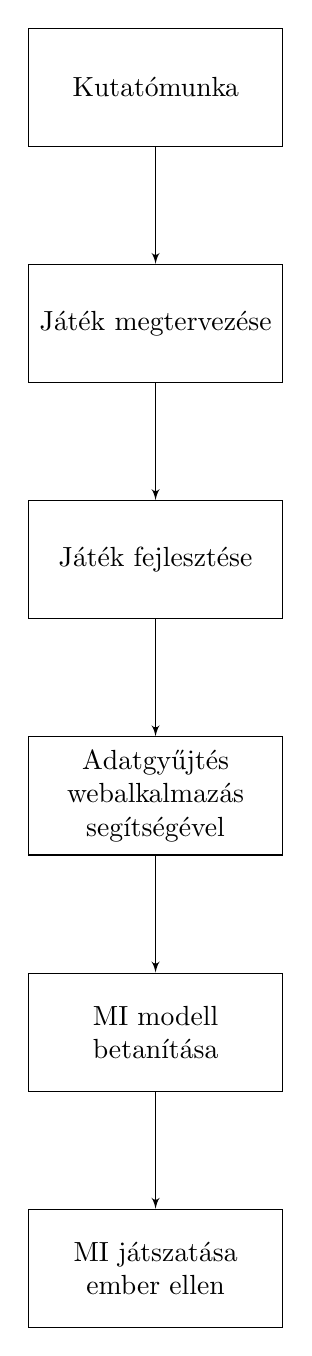
\begin{tikzpicture}[>=latex',node distance=2cm,auto]
        % Define block styles
        \tikzstyle{block} = [rectangle, draw, text width=3cm, text centered, minimum height=1.5cm ]
        \tikzstyle{line} = [draw, -latex']

        % Nodes
        \node [block] (kutatomunka) {Kutatómunka};
        \node [block, below of=kutatomunka, node distance=3cm] (tervezes) {Játék megtervezése};
        \node [block, below of=tervezes, node distance=3cm] (jatek_megirasa) {Játék fejlesztése};
        \node [block, below of=jatek_megirasa, node distance=3cm] (adatgyujtes) {Adatgyűjtés webalkalmazás segítségével};
        \node [block, below of=adatgyujtes, node distance=3cm] (MI) {MI modell betanítása};
        \node [block, below of=MI, node distance=3cm] (MI_ember) {MI játszatása ember ellen};

        % \node [block, right of=section1, node distance=4cm] (subsection1) {Subsection 1};
        % \node [block, right of=section2, node distance=4cm] (subsection2) {Subsection 2};

        % Arrows
        \path [line] (kutatomunka) -- (tervezes);
        \path [line] (tervezes) -- (jatek_megirasa);
        \path [line] (jatek_megirasa) -- (adatgyujtes);
        \path [line] (adatgyujtes) -- (MI); 
        \path [line] (MI) -- (MI_ember);

    \end{tikzpicture}
    \caption{A projekt folyamatábrája}
    \label{fig:folyamat_diagram}
\end{figure}

\subsection{Kutatómunka}
A kutatómunka során elsősorban azt vizsgáltam, hogy melyik tanító algoritmussal érhetem el a kívánt eredményt. Különböző irodalmakat tanulmányoztam, valamint áttekintettem mások munkáit a témában. A kutatómunka végeztével összegeztem a talált eredményeket.

\subsection{Játék megtervezése}
A kutatómunka után el kellett döntenem, hogy milyen játékot fejlesztek, amely elég bonyolult ahhoz, hogy kihívást jelentsen a játékosok számára, ugyanakkor elég egyszerű ahhoz, hogy az AI betanítása belátható időn belül megtörténjen. Ezen a ponton meg kellett azt is határoznom, hogy milyen technológiát alkalmazok, valamint hogy mely területekre összpontosítok a fejlesztés folyamán. A Játék elkészítéséhez a Godot enginen-t választottam.

\subsection{Játék fejlesztése}
A megfelelő tervezés után lefejlesztettem a választott fejlesztői környezetben a játékot. A fejlesztés során két fontos szempontot tartottam szem előtt: a játékot lehetővé kell tenni virtuális valóságban és asztali számítógépen egyaránt, valamint biztosítanom kell, hogy az AI képes legyen kezelni a játékot csupán a játék metainformációinak ismeretében.

\subsection{Adatgyűjtés és VR támogatás}
Miután elkészült a játék, több különböző korosztállyal játszattam azt annak érdekében, hogy elegendő adatom legyen az AI betanításához. Ebben az időszakban foglalkoztam a játék VR támogatásának fejlesztésével is.

\subsection{AI betanítása}
A gyűjtött adatokat felhasználva betanítottam az AI-t egy tanító algoritmus segítségével.

\subsection{AI játszatása}
A játékhoz létrehoztam egy interfészt, amely lehetővé tette az AI számára, hogy játszhasson vele. Miután ez sikeresen működött, lehetőséget teremtettem arra is, hogy az emberi játékos a gép ellen is játszhassa a játékot.